\documentclass[12pt,UTF8]{ctexbook}
\usepackage{ctex}
\usepackage{array}
\usepackage{graphicx}
\usepackage{wrapfig}
\usepackage[table,dvipsnames]{xcolor}
\usepackage{tabularx}
\usepackage{longtable}
\usepackage{float}
\usepackage{amsmath}
\usepackage{amssymb}
\usepackage{xfrac}
\usepackage{eucal}
\usepackage{titlesec}
\usepackage{amsthm}
\usepackage{tikz-cd}
\usepackage{enumitem}
\usepackage{verbatim}
\usepackage{fontspec,xunicode,xltxtra}
\usepackage{xeCJK} 
\usepackage{caption}
\usepackage{thmtools, thm-restate}
\usepackage{mhchem}
% 修改脚注的编号为加圈样式,并且各页单独编号
\usepackage{pifont}
\usepackage[b]{esvect}
\usepackage[perpage,symbol*]{footmisc}
\DefineFNsymbols{circled}{{\ding{192}}{\ding{193}}{\ding{194}}
{\ding{195}}{\ding{196}}{\ding{197}}{\ding{198}}{\ding{199}}{\ding{200}}{\ding{201}}}
\setfnsymbol{circled}

\definecolor{gl}{RGB}{246, 252, 240}
\definecolor{gd}{RGB}{236, 244, 230}
\definecolor{bg}{RGB}{242, 244, 228}

\setCJKmainfont[BoldFont=STZhongsong]{STSong}
\setCJKmonofont{simkai.ttf} % for \texttt
\setCJKsansfont{simfang.ttf} % for \textsf
\setlength\parskip{8pt}
\setlength{\fboxsep}{12pt}
\renewcommand\thesection{\arabic{chapter}.\arabic{section}}
\newcommand{\arccot}{\operatorname{arccot}}
\newcommand{\dlim}[1]{^{\color{gray}\prime}#1}
\newcommand{\lian}[1]{
    \underset{#1}{\operatorname{lian}\,}
}
\newcommand{\di}[1]{\,\mathrm{d}#1}
\newcommand{\qu}[2]{\displaystyle\left(#1;#2\right)}
% developpements limites
\newcommand{\oveq}[1]{\overset{#1}{=}} 
\newcommand{\olim}[1]{\mathit{o}\left(#1\right)}  % petit o
\newcommand{\Olim}[1]{\mathcal{O}\left(#1\right)}  % grand O
\newcommand{\Tlim}[1]{\mathcal{\Theta}\left(#1\right)}  % grand theta
\newcommand{\eqlim}[1]{\overset{#1}{\sim}}  % equivalence
\newcommand{\vect}[1]{\left\langle #1 \right\rangle}

\newcommand{\rectbx}{%
    \mathord{\text{%
        \tikz[baseline] \draw (0,.1ex) -- (.8em,.1ex) -- (.8em,1.5ex) -- (0em,1.5ex) -- cycle;}
    }
}

\theoremstyle{definition}
\newtheorem{df}{定义}[section] 
\newtheorem*{po}{公理}
\newtheorem{pp}{命题}[section]
\newtheorem{tm}{定理}[section]
\newtheorem{cor}{推论}[pp]
\newtheorem{ex}{例子}[section]
\newtheorem{et}{例题}[section]
\newtheorem*{ex*}{例子}
\newtheorem*{so}{解答}
\theoremstyle{plain}
\newtheorem{sk}{思考}[section]
\newtheorem{xt}{习题}[section]
\renewenvironment{proof}{\paragraph{\textbf{证明:}}}{\hfill$\square$}

% 列举环境的行间距
\setenumerate[1]{itemsep=0pt,partopsep=0pt,parsep=0pt,topsep=0pt}
\setitemize[1]{itemsep=0pt,partopsep=0pt,parsep=0pt,topsep=0pt}
\setdescription{itemsep=0pt,partopsep=0pt,parsep=0pt,topsep=0pt}
% 章节字体大小
\titleformat{\section}{\zihao{-2}\bfseries}{ \thesection }{16pt}{}
% 封面
\title{\zihao{0} \bfseries 第五册}
\author{\zihao{2} \texttt{大青花鱼}}
% \date{\bfseries\today}
\date{}
% 正文
\begin{document}
\maketitle
\tableofcontents
\newpage

\chapter{度量和度量以外}

数学的重要研究对象之一,就是平面、空间中的形状。我们从中抽象出了平面形和空间形,定义了点、直线、曲线、平面、三角形、圆形等概念,
通过距离、长度、角度来描述、理解它们的性质。我们构造了向量和平直空间、直变换的概念,来描述、理解平面形、空间形的变化。

另一方面,我们通过研究实变量的函数,对平面中的曲线有了一定了解。通过研究连续函数及其微变率的性质,
我们对作为函数图像的曲线有了基本认识。为了更好地理解平面乃至空间中的形状,我们需要更多的工具。

我们把空间视为点的集合。向量就是描述这些点和空间关系的一种方法。我们通过内积定义了向量的距离、长度、角度,从而可以描述空间中的形状。
我们把这样的空间称为内积空间(即配备了内积的空间)。空间形作为点的集合,可以用距离、长度、角度来描述。

我们把和距离、长度、角度相关的性质称为\textbf{度量性质}。除此之外,空间形作为点的集合,还有其他的性质。
比如,我们讨论函数图像的性质的时候,往往讨论“一点附近”或“无穷远处”的行为。这些概念和具体的长度、距离关系不大。
这些性质对我们理解空间形状的本质十分重要。

\section{邻域、开集和闭集}

为了理解数轴上的点集,我们引进了区间的概念。区间是一种基本的点集。为了研究曲线在一点附近的情况,我们引入了邻域的概念。
邻域可以用来方便地描述“附近”这件事。对于平面上乃至空间中的点集,我们也引入一些基本的概念,帮助我们描述定义在平面和空间上的映射。

从数轴上的区间的概念出发,我们可以定义平面乃至空间上的“区间”:

\begin{df}{\textbf{方区}}
    给定开区间$(a;b)$、$(c;d)$\footnote{其中$a,b,c,d$可以为无穷大。},我们称平面点集:
    $$\{(x, y) \, | \, a < x < b,\, c< x < d\}$$
    为$(a;b)$、$(c;d)$构成的\textbf{开方区},记为$(a;b)\times(c;d)$。

    给定闭区间$[a;b]$、$[c;d]$,我们称平面点集:
    $$\{(x, y) \, | \, a \leqslant x \leqslant b,\, c \leqslant x \leqslant d\}$$
    为$[a;b]$、$[c;d]$构成的\textbf{闭方区},记为$[a;b]\times[c;d]$。

    一般来说,如果有数$a,b,c,d$使得平面点集$S$满足:
    $$(a;b)\times(c;d) \subseteq S \subseteq [a;b]\times[c;d],$$
    就说$S$是$a,b,c,d$构成的方区,记为$\rectbx_{a;b;c;d}$。

\end{df}

直观上,方区就是平面上的长方形区域,其各边分别与坐标轴平行。开方区类似于开区间,是不包括边界的长方形区域;
闭方区则类似于闭区间,是包括了完整边界的长方形区域。

对于区间来说,除了开区间和闭区间,还有半开半闭区间。由于区间的“边界”就是两端点,所以情况简单。对于方区来说,
边界是长方形,所以情况复杂得多。我们笼统地称它们为方区。

同理,我们也可以定义空间中的开、闭方区:
\begin{align*}
    (a_x;b_x)\times(a_y;b_y)\times(a_z;b_z) &= \{(x, y, z) \, | \, a_x < x < b_x,\, a_y < x < b_y,\, a_z < z < b_z\} \\
    [a_x;b_x]\times[a_y;b_y]\times[a_z;b_z]\; &= \{(x, y, z) \, | \, a_x \leqslant  x \leqslant b_x,\, a_y \leqslant x \leqslant b_y,\, a_z \leqslant z \leqslant b_z\}
\end{align*}
其中$a_x, b_x, a_y, b_y, a_z, b_z$等是描述方区范围的数。
一般来说,在$n$维平直空间里,也可以定义
\begin{align*}
    (a_1;b_1)\times(a_2;b_2)\times\cdots\times(a_n;b_n) &= \{(x_1, x_2, \cdots, x_n) \, | \, \forall i\in[1..n],\,\, a_i < x_i < b_i\} \\
    [a_1;b_1]\times[a_2;b_2]\times\cdots\times[a_n;b_n]\; &= \{(x_1, x_2, \cdots, x_n) \, | \, \forall i\in[1..n],\,\, a_i \leqslant x_i \leqslant b_i\} 
\end{align*}
使用方区的概念,我们可以定义平面和空间上的“邻域”。比如数轴上一点$x$有邻域$(x-r;x+r)$,
那么也可以说平面上一点$(x, y)$有开邻域$(x-r;x+r)\times(y-r;y+r)$和闭邻域$[x-r;x+r]\times[y-r;y+r]$。

显然,我们还可以定义别的形状的邻域。比如圆形的开邻域和闭邻域:
\begin{align*}
    \bigcirc_{(x,y)}(r) &= \{(s, t) \, | \, \sqrt{(s - x)^2 + (t - y)^2} < r\} \\
    \overline{\bigcirc}_{(x,y)}(r) &= \{(s, t) \, | \, \sqrt{(s - x)^2 + (t - y)^2} \leqslant r\}
\end{align*}
% $$ \bigcirc_{(x,y)}(r) = \{(s, t) \, | \, \sqrt{(s - x)^2 + (t - y)^2} < r\} $$
这里我们用到了距离和长度的概念:邻域$\bigcirc_{(x,y)}(r)$表示到$(x, y)$的距离小于$r$的点的集合。

以上定义的邻域有什么共性呢?

邻域是用来探讨一点附近的情况的。把集合$S$的元素视为点,邻域就是$S$的子集。我们这样描述一般的邻域:
\begin{enumerate}
    \item 任一点$x$都有邻域,邻域是包含$x$的集合。
    \item 任一点$x$的任何邻域$L$的母集$M$还是$x$的邻域。
    \item 任一点$x$的任何邻域$L$的交集还是$x$的邻域。
    \item 任一点$x$的任何邻域$L$都包含$x$的某个邻域$N$作为真子集,而且$L$是$N$中每一点的邻域。
\end{enumerate}
前三点很好理解。第四点说明:我们从一点出发,可以“稍微动一动”,还在同一个邻域里。
这个特性让我们能够谈论不同点的共同邻域。

集合$S$中所有邻域合称为$S$上的\textbf{邻域结构}。同一个集合$S$可以拥有各种不同的邻域结构。
邻域结构告诉我们集合$S$上点的邻近关系。

以下是一些邻域的例子:
\begin{itemize}
    \item 实数集$\mathbb{R}$中,点$x$的邻域可以是包含它的任何开区间,或包含它且不以它为端点的闭区间。
    \item 区间$[0;1]$中,点$x=1$的邻域可以是$(a;1]$,其中$0\leqslant a < 1$。
\end{itemize}

用这个观点来看开邻域和闭邻域,可以发现:
\begin{itemize}
    \item 开邻域是其中每一点的邻域。从其中每一点出发,总可以“稍微动一动”,还在开邻域里。
    \item 闭邻域“隔开”了其外每一点。从闭邻域外的点出发,总可以“稍微动一动”,而不跑到闭邻域里面去。
\end{itemize}
这两种邻域抽象了“里外”的概念。

举例来说,考虑$x=1$的情况,对于给定的$r$来说,开邻域为$(1-r;1+r)$,闭邻域为$[1-r;1+r]$。

如果我们从$x\in(1-r;1+r)$出发,稍微往右移,可以给它加上$\frac{1+r-x}{2}$,即它到区间右端的一半距离,
这样得到的点还在$(1-r;1+r)$里。而对闭邻域$[1-r;1+r]$来说,由于有端点,如果从端点$1+r$出发往右移,
无论动多少,总会跑到外面去。

从$x>[1-r;1+r]$出发,稍微往左移,可以给它加上$\frac{x-(1+r)}{2}$,即它到区间右端的一半距离,
这样得到的点还在$[1-r;1+r]$外。而对开邻域$(1-r;1+r)$来说,如果从点$1+r$出发往左移,
无论动多少,总会跑到$(1-r;1+r)$里面去。

我们把这种性质推广到一般的点集:
\begin{df}
    如果集合是其中每一点的邻域,就说它是\textbf{开集}。开集的补集称为\textbf{闭集}。
\end{df}

举例来说,在定义了距离和长度的空间里,
给定$r>0$,我们把到一点距离小于$r$的点的集合称为\textbf{开球},把到一点距离小于等于$r$的点的集合称为\textbf{闭球}。
\begin{itemize}
    \item 如果点集$S$中任一点$\mathbf{u}$都能被$S$中某个开球$\bigcirc_{\mathbf{u}}(r)\subseteq S$包含,就说$S$是\textbf{开集}。
    \item 如果$S$在空间中的补集是开集,就说$S$是闭集。
\end{itemize}

显然,开集的定义是直观的。开集允许我们在里面“稍微动一动”,而不跑到集合外面去。定义中要求存在的$r$,就是移动的“安全距离”。
这说明开集中的点都在集合“里面”。比如,按定义,开球就是开集。

空集是否是开集?由于开集的定义是一个假言命题,所以,如果$S$中没有点,那么自动满足开集定义:\textbf{空集是开集}。

闭集则没那么直观,它代表了“外”的概念,因此定义为开集的补集。简单来说,闭集就是“开集的外面”,闭集的“外面”就是相应开集的“里面”。
比如,闭球是闭集,因为可以证明,空间“挖掉”一个闭球后剩下的部分是开集。

在定义了距离和长度的空间里,我们还可以更直观地定义闭集。我们首先引入\textbf{极限点}的概念。极限点是极限的“推广”。
对于序列来说,给定序列$\{a_n\}_{n\in\mathbb{N}}$,
它的子序列的极限就称为它的极限点。直观来说,点列的极限点就是被序列中的点无限逼近、聚拢的点。

类似地,可以定义点集的极限点。给定点集$S$,如果点$x$的任何邻域都包含$S$的元素,就说$x$是$S$的极限点。
换句话说,如果$\forall r>0$,都有$s\in S$使得$s$到$x$的距离小于$r$,这样的$x$就是$S$的极限点。
另一种说法是:如果可以在$S$中找到极限为$x$的序列,那么$x$是$S$的极限点。

要注意的是:如果$x\in S$,那么按定义,包含$x$的任何集合都包含$S$的元素,即$x$自己。因此$S$的元素总是它的极限点。
因此,只要点$x$属于$S$,即便是孤零零一点,也是极限点。

为了排除这种情况,我们定义\textbf{聚点}:
如果点$x$的任何去心邻域\footnote{即从邻域中去掉$x$剩下的集合。}都包含$S$的元素,就说$x$是$S$的\textbf{聚点}。
聚点是我们真正想要描述的:被点集中的点无限逼近、聚拢的点。不是聚点的极限点称为\textbf{孤点}。

点集的聚点不一定在点集里。比如,区间$(0;1)$中可以找出无限逼近$1$的点,但$1$不在$(0;1)$里。可以证明:
\begin{tm}
    如果$S$的聚点总属于$S$,那么$S$是闭集。反之亦然。
\end{tm}

目前来说,我们可以把聚点作为判断闭集的准则。

给定点集$S$,它所有极限点的集合称为$S$的\textbf{闭包}。点集的闭包总是闭集,也总是它的母集,而且是包含$S$的最小闭集。
对于闭集来说,闭包就是它自己;对开集来说则不一定。如果开集的极限点不属于开集,就说它在开集的边界上。
或者说,这样的极限点构成了开集的边界。

点集的最大开子集称为它的\textbf{内部}。点集的内部总是闭包的子集,两者之差称为点集的\textbf{边界}。
显然,开集的内部就是自己,所以开集的边界就是和闭包的差集。闭集的闭包就是自己,所以闭集的边界就是和内部的差集。

点集$S$的闭包记为$\overline{S}$,内部记为$\overset{\circ}{S}$,边界记为$\partial S$。

\section{连续、稠密和紧致}

有了邻域、开集、闭集的概念,我们可以讨论平面、空间中的点的性质。
比如,我们可以把函数在一点连续的定义用邻域来表示:
\begin{df}
    给定函数$f$,$x$是其定义域$D$中一点。如果对$f(x)$的任何邻域$V$,都有$x$的邻域$U$,
    使得
    $$ f(D\cap U) \subseteq V,$$
    就说$f$在$x$处连续。
\end{df}
这个定义不依赖具体的距离、长度、空间,只依赖邻域。

我们甚至可以仅仅用开集来定义连续函数:
\begin{df}
    给定函数$f$,如果$f$的值域中的开集,总是定义域中开集的像,就说$f$是连续函数。
\end{df}




\section{赋长平直空间}

% 从内积空间出发,讨论度量空间和赋长空间

\chapter{广义积合}

\section{一般区间上的积合}

我们已经讨论过闭区间$[a;b]$上连续函数的积合。对于一般的区间、一般的函数,是否能定义积合呢?

\begin{ex}
    \mbox{} \\
    \indent 1. 函数$x\mapsto\frac{1}{x}$在$[0;1]$上是否有积合?\\
    \indent 2. 函数$x\mapsto\frac{1}{x^2}$在$[1;+\infty)$上是否有积合?
\end{ex}

\begin{figure}[h] %this figure will be at the right
    \vspace{4pt}
    \centering
    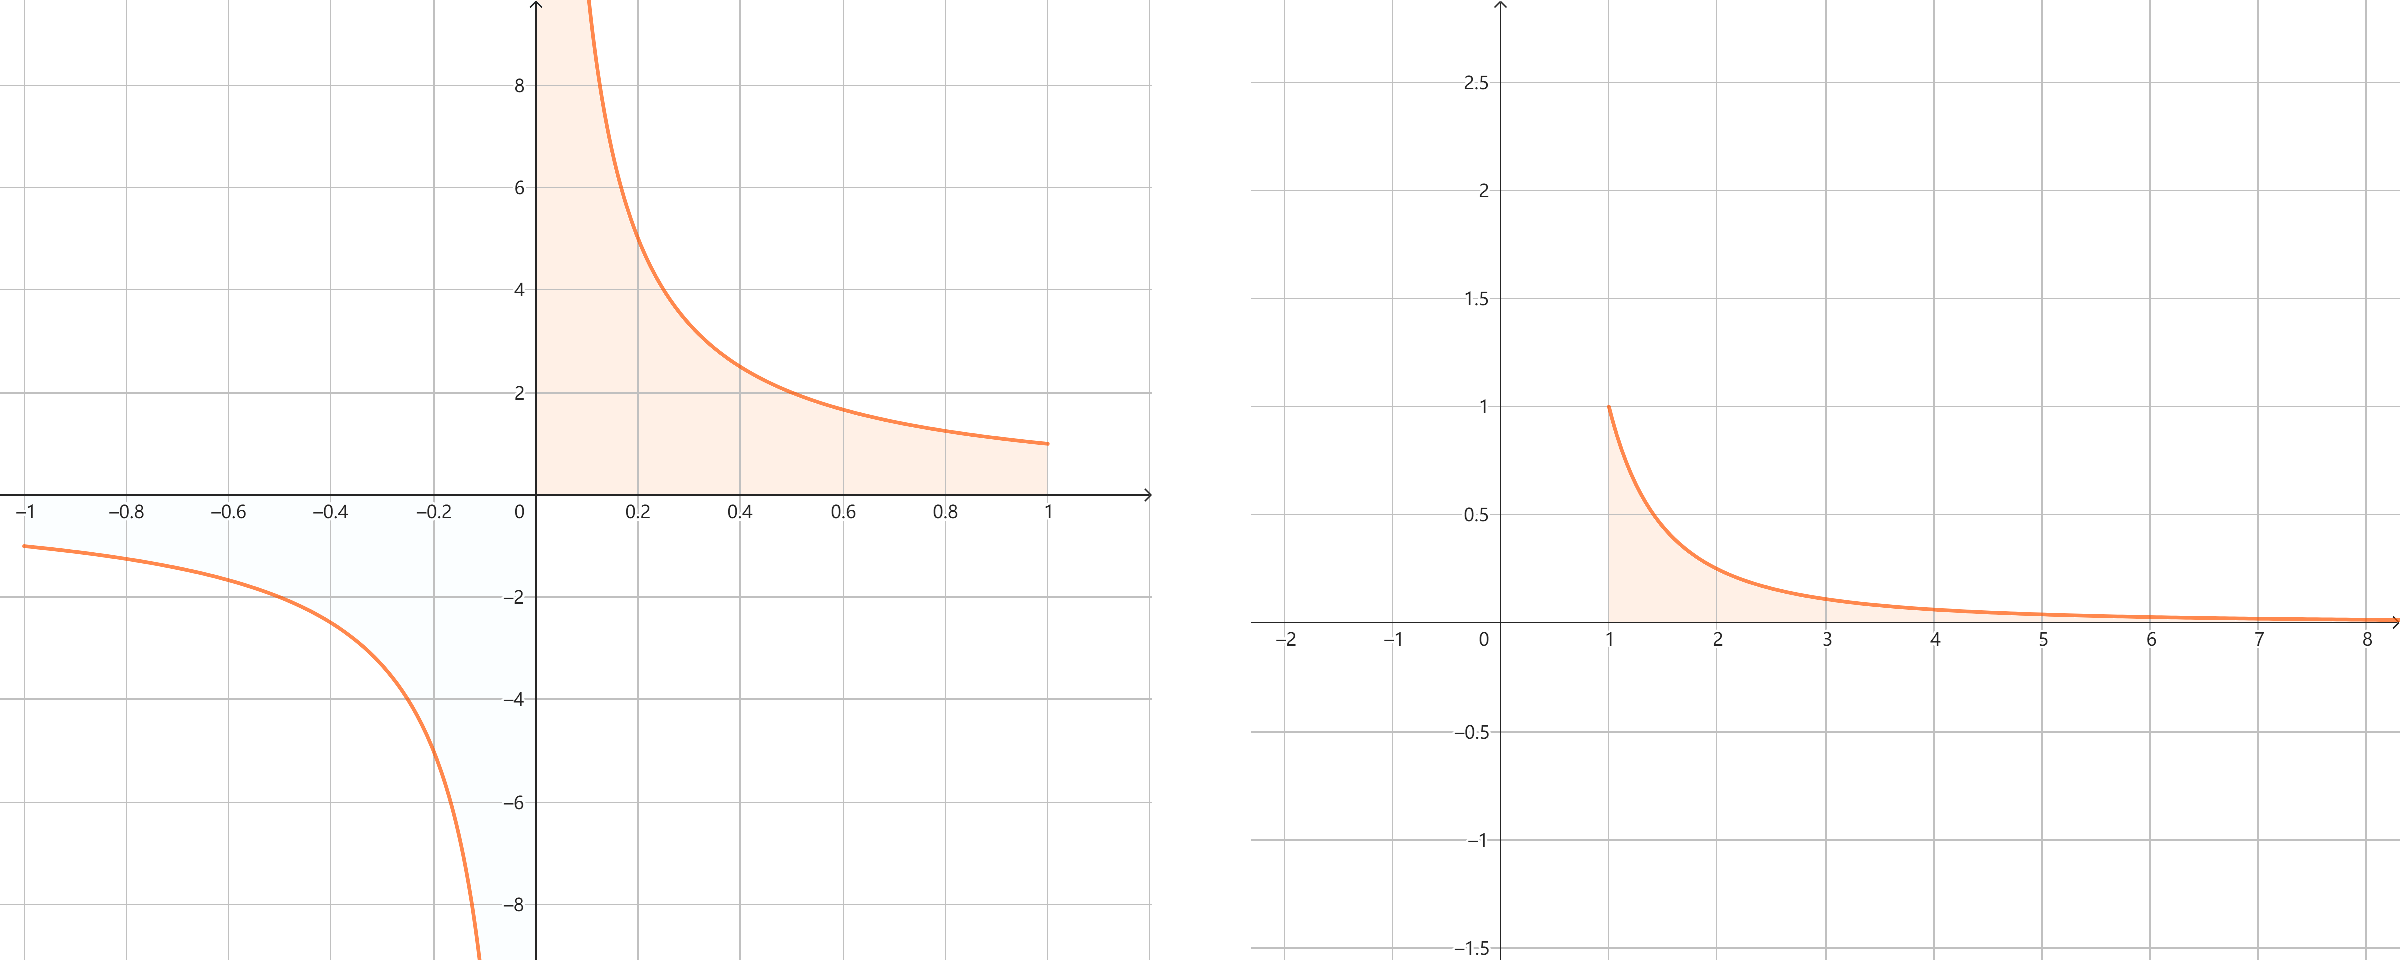
\includegraphics[width=0.9\textwidth]{tu/广义积分1.png}
    \caption*{\texttt{函数}$x\mapsto\frac{1}{x}$(左)、$x\mapsto\frac{1}{x^2}$(右)}
\end{figure}

第一个例子看起来不值得讨论,因为$x\mapsto\frac{1}{x}$甚至不总在$[0;1]$上有定义:$x=0$时,函数无定义。
不过,如果直接看函数的图像,我们能理解这个问题想问什么:如果把积合看作函数与$x$轴之间的图形的面积,那么,
$x\mapsto\frac{1}{x}$这种“无界”的图形是否有面积?

这也是处理一般区间上函数积合时会遇到的问题:闭区间上的连续函数总是有界的,而一般区间上的函数不一定有界。
对于这样的函数,我们能否定义积合呢?

一般来说,以目前的知识,我们无法给任意的函数在任意区间上定义积合。但是,对于一部分“比较好”的函数,我们可以定义积合。

比如,函数$f: x\mapsto\frac{1}{x}$虽然在$[0;1]$上不连续,甚至有未定义的点。但我们可以做一些“修补”。
首先,我们可以给$x=0$处补上定义,比如设$f(0) = 0$。这些工作有助于我们讨论积合的问题,
但不意味着改变函数是否可积的本质。

以上修补过的$f$仍然在$0$处不连续。我们无法直接讨论曲线到$x$轴部分的面积。但我们知道$f$在$(0;1]$上连续。
因此,对任意$a\in(0;1)$,$f$在闭区间$[a;1]$上连续。我们可以求出$f$在$[a;1]$上的面积,然后把$a$趋于$0$。
如果无论$a$以什么方式趋于$0$,面积都趋于一个极限,就定义这个极限为$f$在$[0;1]$上的面积。

首先求$f$在$[a;1]$上的积合:
$$ \int_a^1 f = \ln{1} - \ln{a} = -\ln{a}. $$
这说明$f$在$[a;1]$上的面积是$-\ln{a}$。而$a$趋于$0$时,$-\ln{a}$趋于正无穷。这说明$f$在$[0;1]$上的“面积”是无穷大,
我们说$f$在$[0;1]$上不可积。

第二个例子则比较好理解,因为$f:x\mapsto \frac{1}{x^2}$在$[1;+\infty)$上有定义。我们同样尝试用极限的方式定义函数曲线到$x$轴
的面积。首先求$f$在$[1;a]$上的积合,其中$a>1$:
$$ \int_1^a f = -\frac{1}{a} - (-1) = 1 - \frac{1}{a}. $$
因此$a$趋于正无穷时,$f$在$[1;a]$上的积合趋于$1$。我们说$f$在$[1;+\infty)$上可积。

这样,我们就把积合扩展到定义在一般区间上的连续函数。我们称这种积合为\textbf{广义积合}\footnote{不至于混淆时,也可以简称为积合。}:
\begin{df}
    设函数$f$在半开区间$[a;b)$上连续\footnote{$b$可以是无穷。}。如果当$x$趋于$b$时,$f$在$[a;x]$上的积合总趋于某个极限,
    就说这个极限是$f$在$[a;b)$上的积合,即:
    $$ \int_a^b f = \lian{x\to b^-} \int_a^x f. $$
\end{df}

定义中我们只讨论了区间一端的问题。不过,对于开区间$(a;b)$,我们显然可以先将它截为两段:$(a;c]$、$[c;b)$(其中$c$为区间内任意一点),
然后分别研究这两段是否可积。如果在$(a;c]$、$[c;b)$上都可积,就定义$f$在$(a;b)$上的积合为两段上积合的和。
$$ \int_a^b f = \lian{x\to a^+} \int_x^c f + \lian{x\to b^-} \int_c^x f. $$ 

第一个例子中,我们还“修补”了另一个问题,就是函数在特定点的值的问题。直观来看,函数在单一点是否有定义,或者取不同的值,
不应该改变函数在整个区间上的积合。因为积合是曲线到$x$轴的面积,是一个整体性质。

为此,我们引入分段连续函数的定义:
\begin{df}{\textbf{分段连续函数}}
    设函数$f$在区间$I$上有定义。如果能找到$I$的分割$x_0, x_1, \cdots, x_n$\footnote{其中$x_0$、$x_n$可以是无穷。},
    使得$f$在各个子区间$(x_i;x_{i+1})$上都连续,就说$f$在$I$上(关于该分割)\textbf{分段连续}。
\end{df}
显然,连续函数不论如何分割,总是分段连续的。但也有函数只分段连续而不在整个区间上连续。
比如我们见过的阶梯函数,就是分段连续的不连续函数。

对于分段连续函数,我们可以通过逐段检查,确定它是否可积,并且求出积合。

容易验证广义积合仍然满足积合的基本性质:
\begin{enumerate}
    \item 如果$f$在$I$上可积,且$f$在有限个点以外都大于等于$0$,则其积合大于等于$0$。
    \item 设$a$、$b$、$c$是数轴上的三点,则$\int_a^b f + \int_b^c f = \int_a^c f$。
    \item 设$f$、$g$在$I$上可积,$a, b$为系数,则$ a \int_I f + b \int_I g = \int_I (af + bg) $。
    \item 函数$x\mapsto f\left(\frac{x}{c}\right)$在$[ac; bc]$上的积合,等于$c\int_a^b f$。
    \item 函数$x\mapsto f(x-c)$在$[a+c;b+c]$上的积合,等于$\int_a^b f$。
    \item 如果$f$在区间上的值总介于$m$、$M$之间,那么$m(b - a) \leqslant \int_a^b f \leqslant M(b - a)$。
\end{enumerate}

如果$f$在$I$上有界,那么它在$I$上的广义积合就是它在$I$上的积合。

广义积合与微变也有互逆的关系。比如说,如果$f$在$(a;b]$上可微,且在$a$有右极限,那么:
$$ \int_a^b \partial f = f(b) - \lian{x\to a^+} f.$$
类似地,如果$f$在$[a;b)$上可微,且在$b$有左极限,那么:
$$ \int_a^b \partial f = \lian{x\to b^-} f - f(a).$$

\begin{sk}
    \mbox{} \\
    \indent 1. 函数在一点$a$附近(不包括$a$)连续,它在$a$处不连续。不连续的情况可以分成哪几种?其中哪些可以“修补”成连续函数?\\
    \indent 2. 为什么说函数在有限个点上的取值不影响它在区间上的积合?函数在无限个点上的取值是否影响呢?给定区间$I$的子集$D$,
    你认为当$D$满足什么条件的时候,$f$在$D$上的取值会影响它在区间上的积合?\\
    \indent 3. 小明认为,$x\mapsto\frac{1}{x}$在$(0:1]$上的面积是正无穷,在$[-1;0)$上面积是负无穷,所以在$[-1;1]$上面积为$0$。你怎么看?
\end{sk}

\begin{xt}
    \indent 1. 计算以下积合。$a$趋于给定值时,积合是否收敛?\\    
    \begin{align*}
        1).& \int_a^{1} \frac{\ln{x}}{x} , \; a\to 0^+  &2).& \int_1^{a} e^{-x},  \; a\to +\infty \\[3pt]
        3).& \int_0^{a} \frac{1}{\sqrt{1 - x^2}}, \; a\to 1^-   & 4).& \int_a^{1} \sin{\frac{1}{x}}, \; a\to 0^+ 
    \end{align*}
    \indent 2. 计算以下广义积合。\\    
    \begin{align*}
        1).& \int_0^{+\infty} \frac{1}{x\ln^2{x}} ,  &2).& \int_0^{+\infty} xe^{-x^2} \\[3pt]
        3).& \int_0^{+\infty} \frac{1}{(1 + e^{x})^2},  & 4).& \int_0^{+\infty} \frac{e^{-\sqrt{x}}}{\sqrt{x}}
    \end{align*}
    \indent 3. 仿照极限的定义,具体写出“连续函数在$[1;+\infty)$上可积”的定义。\\

\end{xt}

%%% 
\section{广义可积函数}

下面来看一些经典函数的广义积合。

首先来看函数在某点附近不连续导致的广义积合。

考虑函数$x\mapsto x^{-a}$,其中$a>0$为系数。它在$0$处无定义,在$0$右侧趋于正无穷。它是否在$(0;1]$上可积?

对$t>0$,计算它在$[t;1]$上的积合。$a=1$时,我们知道函数不可积。$a\neq 1$时,
\begin{align*}
    \int_t^1 x^{-a} = \frac{1^{1-a}}{1 - a} - \frac{t^{1-a}}{1 - a} = \frac{1 - t^{1-a}}{1-a} 
\end{align*}

$a<1$时,随着$t$趋于$0$,$t^{1-a}$趋于$0$,因此函数在$(0;1]$上可积,积分为$\frac{1}{1-a}$。

$a>1$时,随着$t$趋于$0$,$t^{1-a}$趋于无穷,因此函数在$(0;1]$上不可积。

考虑函数$x\mapsto \ln{x}$,它在$0$处无定义,在$0$右侧趋于正无穷。它是否在$(0;1]$上有积合?

对$t>0$,计算它在$[t;1]$上的积合。
\begin{align*}
    \int_t^1 \ln{x} = 1\cdot \ln{1} - 1 - (t\cdot\ln{t} - t)= t - t\ln{t} - 1
\end{align*}

$t$趋于$0$时,$t\ln{t}$趋于$0$。因此函数在$(0;1]$上可积,积分为$-1$。

再来看函数在无穷区间上的广义积合。

考虑函数$x\mapsto x^{-a}$,其中$a>0$为系数。它是否在$[1;+\infty)$上可积?

对$t>1$,计算它在$[1;t]$上的积合。

$a=1$时,
\begin{align*}
    \int_1^t x^{-a} = \ln{t} - \ln{1} = \ln{t} 
\end{align*}
$t$趋于无穷时,$\ln{t}$趋于无穷,因此函数在$[1;+\infty)$上不可积。

$a\neq 1$时,它在$[1;t]$上的积合为:
\begin{align*}
    \int_1^t x^{-a} = \frac{t^{1-a}}{1 - a} - \frac{1^{1-a}}{1 - a} = \frac{t^{1-a} - 1}{1-a} 
\end{align*}
$a<1$时,随着$t$趋于无穷,$t^{1-a}$趋于无穷,因此函数在$[1;+\infty)$上不可积。

$a>1$时,随着$t$趋于无穷,$t^{1-a}$趋于$0$,因此函数在$[1;+\infty)$上可积,积分为$\frac{1}{a-1}$。

考虑函数$x\mapsto a^x$,其中$a\in(0;1)$为底数。它是否在$[0,\infty)$上可积?

对$t>0$,计算它在$[0;t]$上的积合。
\begin{align*}
    \int_0^t a^x = \frac{a^t}{\ln{a}} - \frac{a^0}{\ln{a}} = \frac{a^t - 1}{\ln{a}}
\end{align*}
随着$t$趋于无穷,$a^t$趋于$0$,因此函数在$[0,\infty)$上可积,积分为$-\frac{1}{\ln{a}}$。

\begin{figure}[h] %this figure will be at the right
    \vspace{4pt}
    \centering
    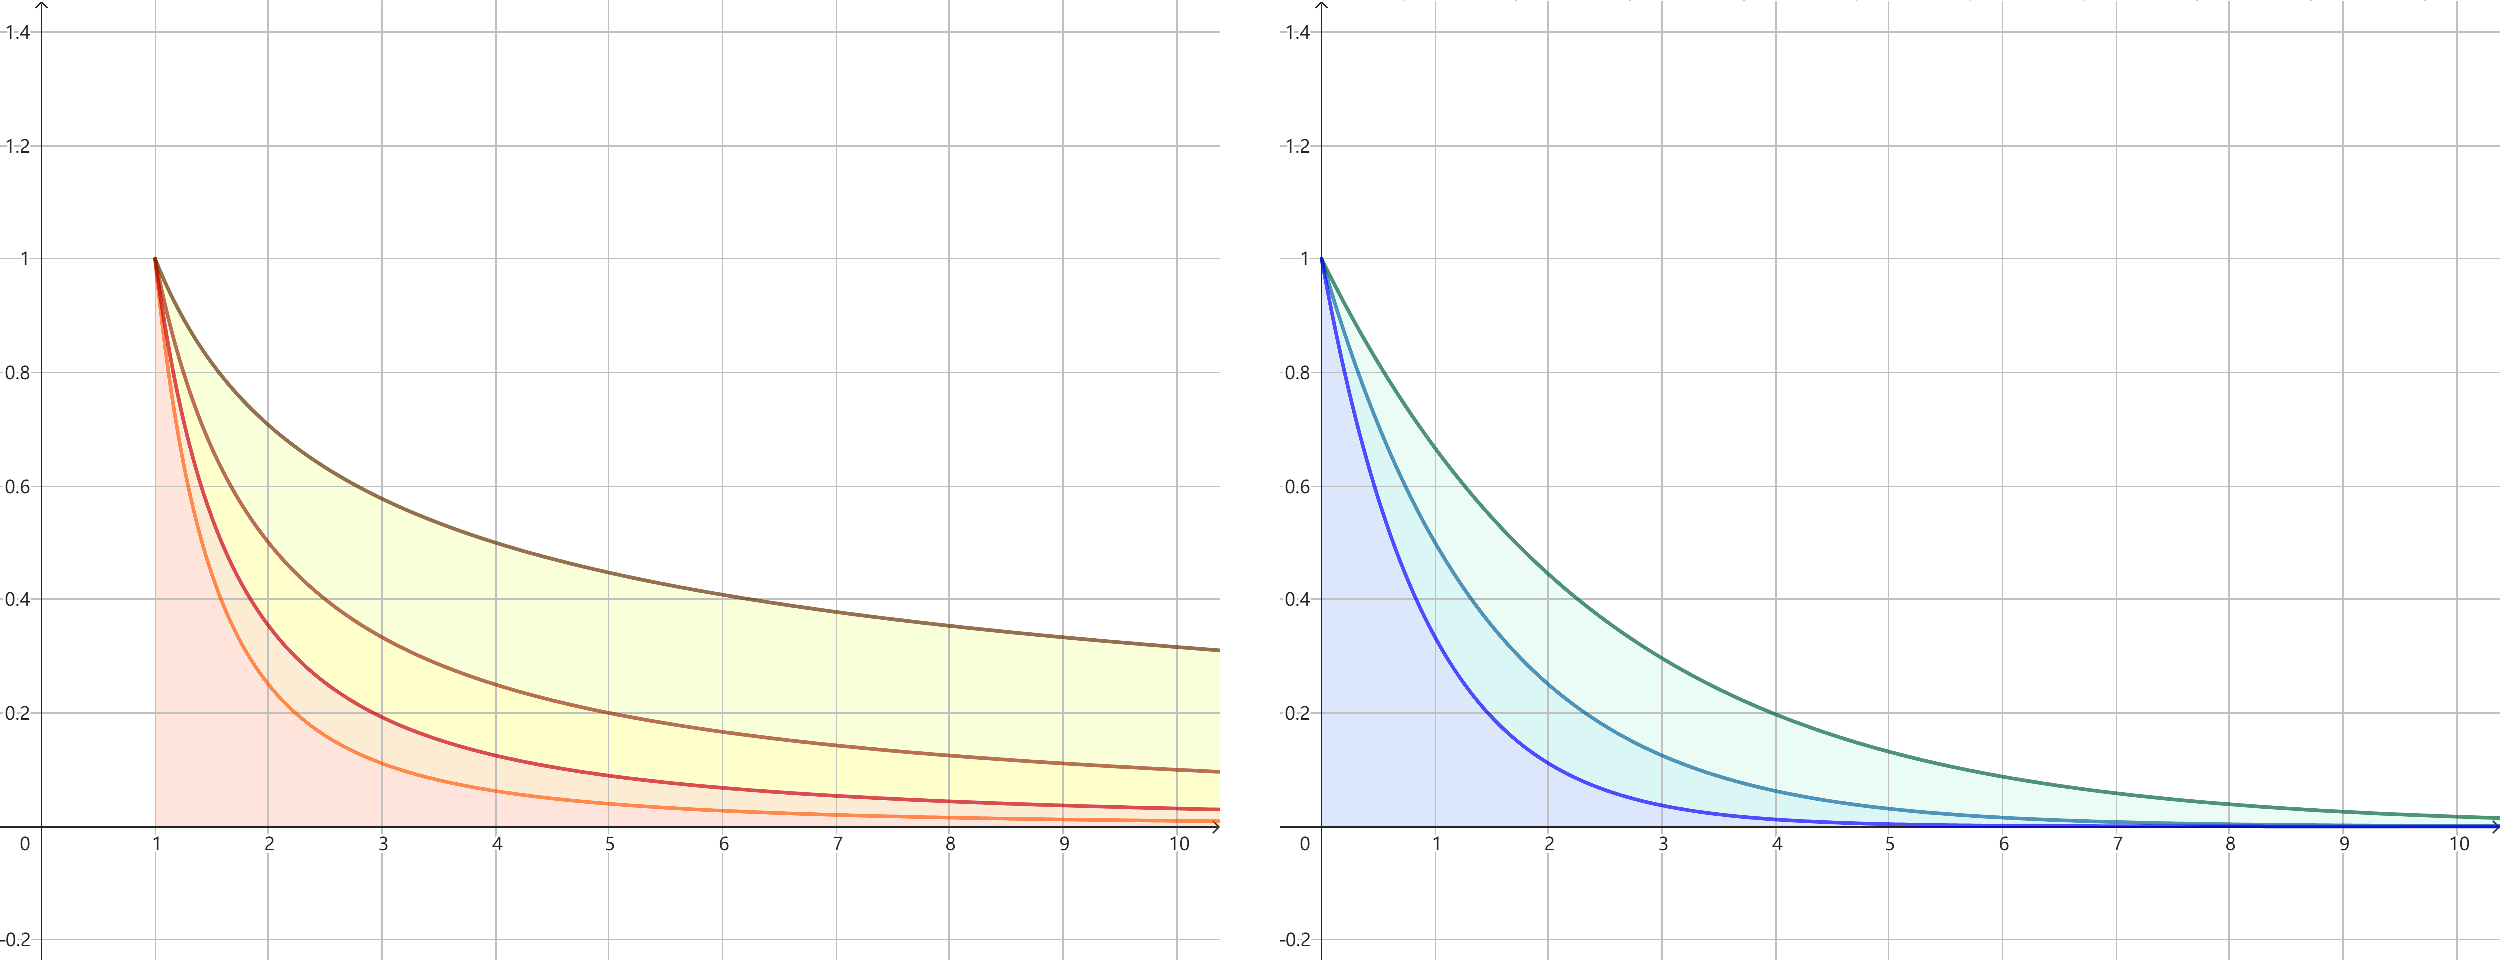
\includegraphics[width=\textwidth]{tu/广义积分2.png}
    \caption*{\texttt{左图:幂函数在}$[1;+\infty)$\texttt{上的面积;右图:指数函数在}$[0;+\infty)$\texttt{上的面积}}
\end{figure}

以上是关于基本的经典函数的讨论,对于更复杂的函数,如何判定它是否广义可积呢?

观察以上的函数在开区间“边缘”的情况,可以发现,造成开区间上面积“无穷”问题的,要么是函数值在开区间端点附近趋于无穷,
要么是开区间为无穷区间——区间长度“无穷”。

我们把前一种情况称为\textbf{无界积合}或\textbf{瑕积合},
把造成问题的端点称\textbf{无界点}或\textbf{瑕点}。而区间为无穷区间的情况,我们称为\textbf{无限积合}。

对于无界积合,直观来说,函数值在瑕点附近急速“爬升”或者“坠落”。
“升”或“落”得越急,曲线到$x$轴的面积就越大;如果“升”或“落”得“太快”,面积就容易变成无穷。

因此,我们可以将函数在无界点附近行为和以上计算过的经典函数进行比较。
如果函数在无界点附近或比可积的经典函数还“慢”,那么可积;如果比不可积的函数还“快”,那么不可积。
而“快慢”程度可以用无穷的阶来具体刻画。

\begin{tm}
    设函数$f$、$g$在区间$I=(a;b]$上分段连续,且在$a$附近同时趋于正无穷。
    \begin{enumerate}
        \item 如果在$a$附近总有$0\leqslant f \leqslant g$,那么只要$g$在$I$上可积,$f$就在$I$上可积。
        \item 如果在$a$附近总有$0\leqslant g \leqslant f$,那么只要$g$在$I$上不可积,$f$就在$I$上不可积。
        \item 如果$f \oveq{a} \Olim{g}$,那么只要$g$在$I$上可积,$f$就在$I$上可积。
        \item 如果$g \oveq{a} \Olim{f}$,那么只要$g$在$I$上不可积,$f$就在$I$上不可积。
        \item 如果$f \oveq{a} \Tlim{g}$,那么$f$在$I$上可积,当且仅当$g$在$I$上可积。
    \end{enumerate}
\end{tm}

举例来说,考虑$(0;1]$上的分段连续函数$f$。如果$f$在$0$点右侧趋于正无穷,那么我们可以将$f$和$x\mapsto x^{-p}$比较。
如果有$p<1$和$r>0$使得$0<x<r$时$f$总受制于$x^{-p}$:
$$ \forall 0<x<r ,\,\,\,\frac{f(x)}{x^{-p}} < M,$$
其中$M$是比值的上界,那么由于$x\mapsto x^{-p}$在$(0;1]$上可积,$f$也在$(0;1]$上可积。

反之,如果$x\mapsto x^{-1}$在$0$右侧附近受制于$f$:
$$ \forall 0<x<r ,\,\,\,\frac{f(x)}{x^{-1}} > M,$$
那么由于$x\mapsto x^{-1}$在$(0;1]$上不可积,$f$也在$(0;1]$上不可积。

再来看无穷积合的情况。
对于无限积合,在无穷远处,如果函数不收敛到$0$,而是收敛到非$0$的数或者趋于无穷,那么显然不可积。
如果函数在无穷远处收敛到$0$,是否就可积呢?

如果函数值(在自变量$x$足够大时)总是正数(或者$0$),那么我们有类似的结论:
\begin{tm}
    设函数$f$、$g$在区间$I=[a;+\infty)$上分段连续。
    \begin{enumerate}
        \item 如果总有$0\leqslant f \leqslant g$,那么只要$g$在$I$上可积,$f$就在$I$上可积。
        \item 如果总有$0\leqslant g \leqslant f$,那么只要$g$在$I$上不可积,$f$就在$I$上不可积。
        \item 如果$0\leqslant f \oveq{+\infty} \Olim{g}$,那么只要$g$在$I$上可积,$f$就在$I$上可积。
        \item 如果$0\leqslant g \oveq{+\infty} \Olim{f}$,那么只要$g$在$I$上不可积,$f$就在$I$上不可积。
        \item 如果$0\leqslant f \oveq{+\infty} \Tlim{g}$,那么$f$在$I$上可积,当且仅当$g$在$I$上可积。
    \end{enumerate}
\end{tm}

考虑$[1;+\infty)$上的分段连续函数$f\geqslant 0$。我们可以将$f$和$x\mapsto x^{-p}$比较。
如果有$p>1$和$A>0$使得$x>A$时$f$总受制于$x^{-p}$:
$$ \forall x>A ,\,\,\,\frac{f(x)}{x^{-p}} < M,$$
其中$M$是比值的上界,那么由于$x\mapsto x^{-p}$在$[1;+\infty)$上可积,$f$也在$[1;+\infty)$上可积。

反之,如果$x\mapsto x^{-1}$在$0$右侧附近受制于$f$:
$$ \forall x>A ,\,\,\,\frac{f(x)}{x^{-1}} > M,$$
那么由于$x\mapsto x^{-1}$在$[1;+\infty)$上不可积,$f$也在$[1;+\infty)$上不可积。

以上讨论中我们加上了函数大于等于$0$的条件。如果函数值可正可负时,情况更加复杂。
我们可以把无限积合与可数个数求和——也就是级数——的情况类比。
讨论级数收敛时,我们将级数分为正项级数和一般的级数,并引入了级数的绝对值、绝对收敛和相对收敛的概念。

对于无限积合,我们引入\textbf{绝对可积}的概念。
对于定义在区间$I$上的函数$f$,如果它的绝对值$|f|: x\mapsto |f(x)|$在$I$上可积,就说$f$绝对可积;
否则就说$f$\textbf{相对可积}。

在$I$上绝对可积的函数,一定相对可积,但反之则不一定。

要注意的是,如果函数在无穷远处没有极限,并不能说明它可积或不可积。比如说,我们可以在足够远处给函数加上一些“小尖刺”。
每个“小尖刺”的面积都很小,不影响可积,但“刺尖”的函数值可以很大,甚至趋于无穷。

具体来说,我们制作这样的“尖角函数”:
\begin{align*}
    f: [0;1] &\rightarrow \mathbb{R} \\
x \;&\mapsto \begin{cases}
    2x & 0\leqslant x \leqslant \frac{1}{2} \\
    1 - 2x & \frac{1}{2} < x \leqslant 1
\end{cases} 
\end{align*}
这个函数的图像是平放在$x$轴上的等腰三角形。它的左端和$0$对齐,底和高都是$1$。我们可以将它拉伸放缩为“尖刺”:
\begin{align*}
   [a;a+b] &\rightarrow \mathbb{R} \\
    x \;&\mapsto h\cdot f\left(\frac{x-a}{b}\right)
\end{align*}
这个函数的图像也是$x$轴上的等腰三角形,只不过底边是$x$轴上的线段$[a;a+b]$,底长为$b$,高为$h$。

取一个在$[1;+\infty)$上可积的非负函数,比如$f_0: x\mapsto x^{-2}$。在足够远的地方放置这些“尖刺”,得到以下函数:
$$
g: x\mapsto \begin{cases}
    \displaystyle f_0(x) + 2n f\left(n^3(x - n)\right) & \mbox{如果}\; x \in \left[n;n+\frac{1}{n^3}\right],\; n\in\mathbb{Z}^+ \\
    f_0(x) & \mbox{其他的}\;x
\end{cases}
$$
对任意正整数$n$,函数$g$在区间$\left[n;n+\frac{1}{n^3}\right]$上叠加放置了底边为$\frac{1}{n^3}$,高为$2n$的等腰三角形。它的面积为$\frac{1}{n^2}$。

因此,相对于$f_0$,$g$的面积增加不超过$\sum \frac{1}{n^2}$。而$\sum \frac{1}{n^2}$是收敛的级数,所以函数$g$也是可积乃至绝对可积的。
然而,$g$的函数值在$n+\frac{1}{2n^3}$处可以达到$2n$,因此没有上限,随着$n$的增大而趋于无穷。

从这个例子可以看出,无限积合的判断比无界积合、级数收敛的判断更复杂。这是由实数集的不可数特性和函数的复杂性决定的。

\begin{sk}
    \mbox{} \\
    \indent 1. 总结非负连续函数的无限积合和正项级数的收敛的相似性。\\
    \indent 2. 为什么讨论无界积合时,没有考虑函数值的正负性?\\
    \indent 3. 广义积合可以看作对函数的积合求极限。是否可以先对函数求极限,再求积合?这两种操作是否等价?\\
    \indent 4. 连续函数在无穷远处不收敛到$0$,是否一定不可积?
\end{sk}

\begin{xt}
    \mbox{} \\
    \indent 1. 以下函数是否在$\mathbf{R}^+$上可积?\\    
    \begin{align*}
        1).& \frac{1}{x\ln^2{x}} ,  &2).& \frac{e^{-x^2}}{\sqrt{x}} \\[3pt]
        3).& \sin{\frac{1}{x}},  & 4).& \frac{1}{e^x  - 1}
    \end{align*}
    \indent 2. 以下积合是否存在?\\    
    \begin{align*}
        1).& \int_2^{+\infty} \frac{1}{\sqrt{x(x - 1)(x - 2)}}  &2).& \int_0^{\frac{\pi}{2}} \frac{1}{\sin{x}\cos{x}(1 - e^{-x})} \\[3pt]
        3).& \int_0^{1} \frac{\ln{x}}{(1 - x^2)^{\frac{3}{2}}}  & 4).& \int_0^{\pi} \frac{1}{\sqrt{\sin{x}}}
    \end{align*}
    \indent 3. $f$是$[1;+\infty)$上的分段连续函数。\\
    \indent 3.1. 证明:如果有正实数$a>1$使得$\lian{t\to+\infty} t^a f(t) = 0$,那么$f$在$[1;+\infty)$上绝对可积。\\
    \indent 4.2. 证明:如果有正实数$c$使得$\lian{t\to+\infty} t f(t) \geqslant c$,那么$f$在$[1;+\infty)$上不可积。\\
    \indent 4. $f$是$(0;1]$上的分段连续函数。\\
    \indent 4.1. 证明:如果有正实数$a<1$使得$\lian{t\to 0^+} t^a f(t) = 0$,那么$f$在$(0;1]$上绝对可积。\\
    \indent 4.2. 证明:如果有正实数$c$使得$\lian{t\to 0^+} t f(t) \geqslant c$,那么$f$在$(0;1]$上不可积。\\
    \indent 5. 当$a$取什么值的时候,以下带参数$a$的函数在$\mathbb{R}^+$上可积?\\
    \begin{align*}
        1).& \frac{\ln{x}}{x^a} ,  &2).& \frac{e^{-x} - 1}{x^a} \\[3pt]
        3).& \frac{x - \sin{x}}{x^a},  & 4).& \frac{\arctan{x}}{x^a} 
    \end{align*}
    \indent 6. 设$f$是$\mathbb{R}^+$上的连续可积函数。\\
    \indent 6.1. 设$\{x_n\}$、$\{y_n\}$为两个趋于正无穷的数列。证明:
    $$ \lian{n\to+\infty}\int_{x_n}^{y_n} f = 0. $$
    \indent 6.2. 证明:$e^{-t\sin{t}}$在$\mathbb{R}^+$上不可积。

\end{xt}



\end{document}